\section{Rank 3 States}
In this section, we discuss the results of ``breaking" absolute separability via quantum switch. Here, by ``breaking" we mean having a separable state from a AS state via global unitary. We start by considering a very simple case to see if it is at all possible. In a bipartite qubit system, let us consider an AS state. Note that, the rank of the state can either be $3$ or $4$. 
    Let us consider a rank $3$ AS state $\rho_{AB}=\frac{1}{3} (\ket{00}\bra{00}+\ket{01}\bra{01}+\ket{10}\bra{10})$ which lies on the boundary of the convex set in $2\otimes 2$ dimension. Under the switching action of two global unitaries, one being CNOT gate and the other given by, 
    \begin{equation}
        U = 
    \begin{pmatrix}
        cos\theta & 0 & 0 & sin\theta\\
        0 & cos\theta & sin\theta & 0\\
        0 & sin\theta & -cos\theta & 0\\
        sin\theta & 0 & 0 & -cos\theta
    \end{pmatrix},
    \label{unitary_theta}
    \end{equation}
    the resulting state is not an AS state.    We know that the CNOT gate in the computational basis is described by,
    \begin{equation}
    V_{CNOT}= \left(
    \begin{array}{cccc}
     1 & 0 & 0 & 0 \\
     0 & 1 & 0 & 0 \\
     0 & 0 & 0 & 1 \\
     0 & 0 & 1 & 0 \\
    \end{array}
    \right)
    \end{equation}
    Now, following Eq.(\ref{finalstate_switch}) with the initial state as $\rho_{AB}$, one can obtain the final state where $\mathcal{U}_1$ and $\mathcal{U}_2$ are CNOT and $U$. The eigenvalues of the final state, arranged in a non-increasing manner are given by, $\{ \frac{4}{3(3+cos2\theta)}, \frac{1}{3}, \frac{2(1+cos2\theta)}{3(3+cos2\theta)},0 \}$. Let us consider the final state obtained is also an AS state. Hence with the given set of eigenvalues, we construct the criterion to identify AS states. Note that, with these eigenvalues, the inequality in Eq. (\ref{AS_eigenvalue}) reduces to $\cos{(2\theta)}\geq 1$, which is itself contradictory. So our assumption is not correct and it implies that the final state is residing outside the set of AS states in the given dimension. Now with PPT criterion, we verify that the state is a separable state. Hence we obtain a separable state starting from an AS state.
\section{Werner States}
Werner formulated mixed state entanglement in a mathematically rigorous framework
and discovered that there are quantum states which exhibit entanglement but no nonlocality [13],
that is, while any separable state can be modeled by a hidden-variable theory and hence satisfies all
generalized Bell inequalities, the converse is not true. This was achieved by a class of quantum states
introduced by Werner in an ingenious way, and now named after him [13]. Since then, the Werner
states, due to their fundamental characteristics and nice features, have been extensively studied and
widely used in quantum information [14–46]. Despite their seemingly simple structure, the Werner
states and their various generalizations exhibit very rich correlations, ranging from separability to
entanglement, from steering to nonlocality, depending on the single intrinsic parameter in the Werner states [31]. Quantitative knowledge and precise engineering of the two-qubit Werner states have rendered these states as a paradigm for both theoretical and experimental explorations of quantum
information. The Werner states (which are mixed in general), together with the Bell states (which
are pure), constitute a popular playground in studying quantum correlations.
Apart from the Bell states, the Werner states are the most prominent examples of bipartite states
and offer a unique testing ground for quantum information investigations. The Werner states on a
bipartite system Hilbert space $\mathcal{H} \otimes \mathcal{H}$ with dim$\mathcal{H}$ = d have at least three representations [13]:
(1) Werner states as linear combination of the identity operator and the swap operator. In this
representation, the Werner states are defined as
\begin{equation*}
    w=\frac{d-x}{d^3-d}\mathbf{I}\otimes\mathbf{I} + \frac{dx-1}{d^3-d}F,\hspace{1cm} x \epsilon [-1,1]
\end{equation*}
where 1 is the identity operator on H, and F is the swap operator on H $\otimes$ H defined as 
\begin{equation*}
    F(\ket{\psi} \otimes \ket{\psi}) = \ket{\psi} \otimes \ket{\psi}, \hspace{1cm} \forall \ket{\psi}, \ket{\psi} \epsilon \mathcal{H}    
\end{equation*}
Explicitly,
\begin{equation*}
    F = \sum^{d}_{\mu,\nu=1} \ket{\mu}\bra{\nu} \otimes \ket{\nu}\bra{\mu},
\end{equation*}
which is independent of the choice of the orthonormal basis {$\ket{\mu}$ : $\mu$ = 1, 2, · · · , d} of H. Clearly,



\subsection{Modified Werner States}
The modified Werner state \cite{W_89} can be written as, 
\begin{equation}
    \rho_W = p \ket{\xi}\bra{\xi}+ \frac{1-p}{4} \mathcal{I}_{4 \times 4}
    \label{mod_Wstate}
\end{equation}
where $\ket{\xi}$ being a pure state of the form, $\ket{\xi} = \cos{\gamma}\ket{00} + e^{i\phi} \sin{\gamma}\ket{11}$, with $0 \leq p \leq 1$, $0 \leq \gamma \leq \pi$ and $0 \leq \phi \leq 2\pi$. It is already well established that the state in Eq. (\ref{mod_Wstate}) is AS for the range $0\leq p \leq \frac{1}{3}$ and it is separable in the region $\frac{1}{3}\leq p\leq \frac{1}{1+2\sin{2 \gamma}}$. Next we move a step further and show that it is possible to achieve separability for a larger region of $p$ when subjected to a global unitary channel via switching order. 
    
\begin{result}
    If the initial state is $\rho_W$ given in Eq.(\ref{mod_Wstate}) and it undergoes the switching operation between two unitary channels, one being CNOT and the other given in Eq. (\ref{unitary_theta}), then it is possible to achieve separability from the region of AS states.
\end{result}

\begin{figure}[htp]
\centering
\fbox{
\subfigure[The eigenvalues of the final state after the switching action on the state in Eq. (\ref{mod_Wstate}) are plotted against the global unitary parameter, $\theta$. Here we consider $p=0.15$ for which  the initial state is AS.]{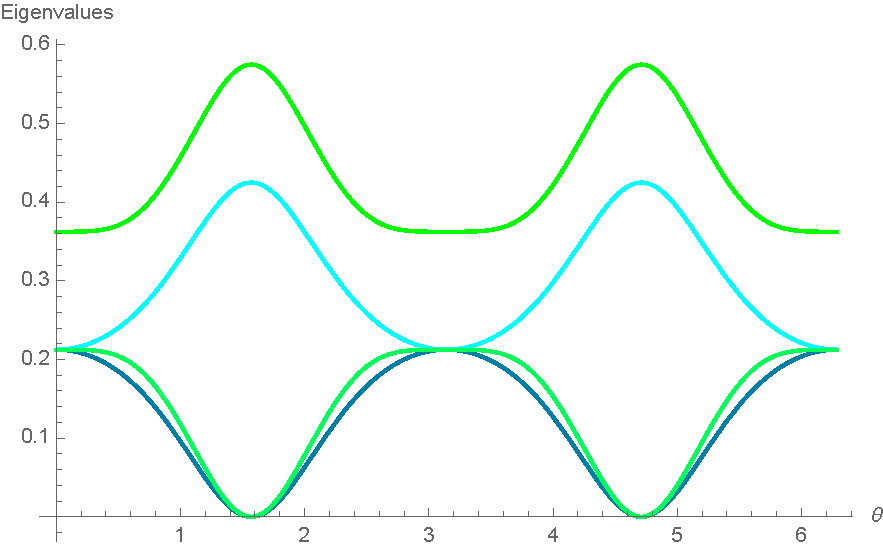
\includegraphics[scale=0.5]{figures/Eigenvalues_modW_f.pdf}}
%\hfill
\qquad
\subfigure[The same eigenvalues are plotted against the noise mixing parameter $p$ ($p$ is varying in the range of AS states) for a fixed $\theta = 1.2$. ]{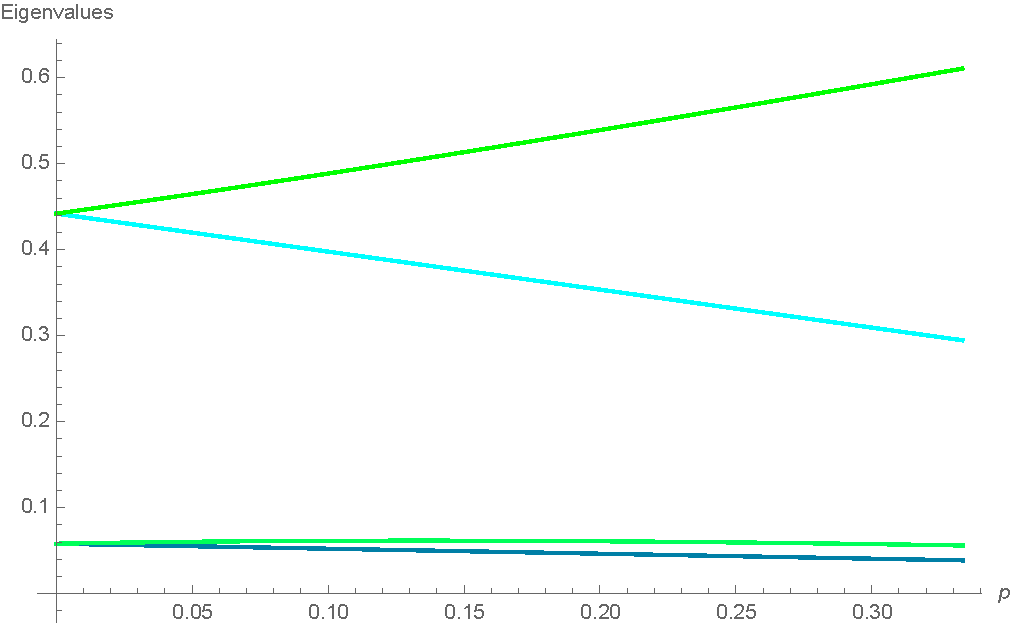
\includegraphics[scale=0.44]{figures/Eigenvalues_modW_f_p.pdf}}}
\caption{\footnotesize{The eigenvalues of the final state}}
\label{eigenvalues_modW}
\end{figure}

    

   \noindent  To prove the statement, we only need to demonstrate an example in which the stated transformation is possible. To begin the demonstration, we observe that the eigenvalues of the initial state in Eq. (\ref{mod_Wstate}) are given by $\{ \frac{1+3p}{4}, \frac{1-p}{4},\frac{1-p}{4},\frac{1-p}{4} \}$, arranged in the non-increasing order. Note that, the eigenvalues are independent of the entanglement content of the pure state $\ket{\xi}$. Now using the process prescribed via Eq. (\ref{finalstate_switch}) with $\mathcal{U}_1=U$ given in Eq. (\ref{unitary_theta}) and $\mathcal{U}_2=CNOT$, we get the eigenvalues of the final state as shown in the Fig. (\ref{eigenvalues_modW}). The eigenvalues are then arranged in non-increasing order for the whole range of the noise mixing parameter $p$ of the state and the unitary matrix parameter $\theta$. 
    
    \begin{figure}[htp]
    \fbox{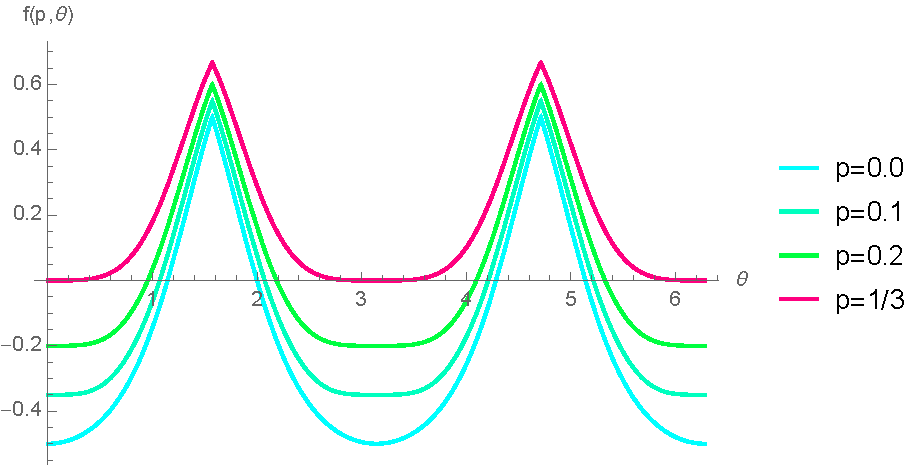
\includegraphics[scale=1]{figures/LHS_eval_cond_modW.pdf}}
    \caption{\footnotesize{The LHS of the eigenvalue condition given in Eq. (\ref{AS_eigenvalue}) is plotted against the unitary matrix parameter for different values of state parameter of AS states.}}
    \label{LHS_eval_cond_modW}
    \end{figure}
    
    In the next step, to check whether the final state remains an AS or not we further evaluate the LHS of Eq. (\ref{AS_eigenvalue}) and obtain the expression as a function of $p$ and $\theta$ (say, $f(p, \theta)$). Plotting this function shows that the condition given in Eq. (\ref{AS_eigenvalue}) is not satisfied for a broad range of $p$ as well as $\theta$ as shown in Fig (\ref{LHS_eval_cond_modW}). Hence for a given choice of unitary it is possible to extend the range of $p$ for which the AS states become separable.
  
   
After proving that it is evidently possible to break absolute separability of modified Werner state via global unitary matrices while employing them with switching order, we look at the results a little bit more carefully. From Fig. (\ref{LHS_eval_cond_modW}) it is clear that for all the values of noise mixing parameter $p$ of the state, there exists certain type of global unitary (corresponding to given values of $\theta$ of $U$ given in Eq. (\ref{unitary_theta})) along with a CNOT gate, which can take out the AS state out of the convex set. Now, looking at Fig (\ref{eigenvalues_modW}.(a)) we see that out of four eigenvalues of the final states, when one becomes $0$ for any value of $p$, another one also goes to $0$. At the same time, the highest eigenvalue takes the largest value. This might happen for several unitary matrices, one being $\theta=\pi/2$ in $U$. Correspondingly, the violation of Eq. (\ref{AS_eigenvalue}) becomes nothing but the largest eigenvalue. For $\theta=\pi/2$, the largest eigenvalue becomes $(1+p)/2$. Note that, the violation hence behaves as a monotonically increasing function of the noise mixing parameter $p$. Interesting even for $p=0$, when the corresponding initial state is a maximally mixed state, it is possible to have the condition for absolute separability violated for certain $\theta$. We emphasise here on the fact that the maximally mixed state $\mathcal{I}/4$ (in $2\otimes2$), which is a free state in every resource theory, it is possible to make it a separable state if one has access to global unitary operations making the initial state resourceful. On the other hand for $p=1/3$, the modified Werner states lie in the boundary of AS states, on the verge of becoming separable. Hence, intuitively it can be assumed that these are the states that are the easiest to take out from the set of convex states containing the AS states. Our result confirms the same as it can be seen from the plot in Fig. (\ref{LHS_eval_cond_modW}) that the choice of effective unitary is extensively high. 
%({\color{red}mention something about rank??!!!})

\begin{figure}[htp]
\centering
\fbox{
\subfigure[For $p=0$ (maximally mixed state)]{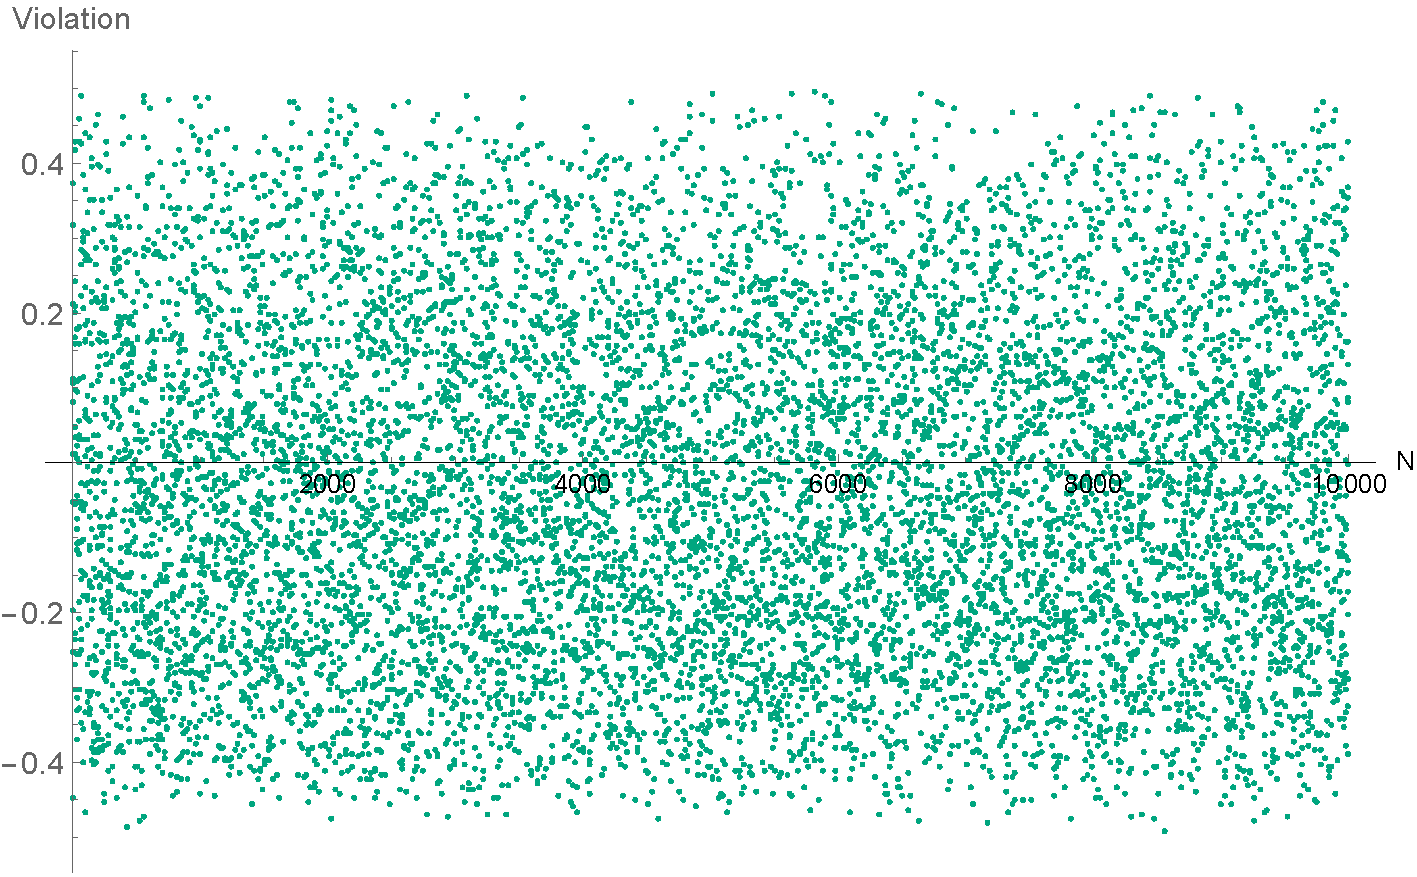
\includegraphics[scale=0.3]{figures/RandomU_p0_10k.pdf}}
%\hfill
\qquad
\subfigure[For $p=1/3$, $\phi=0$, and $\gamma=\pi/4$]{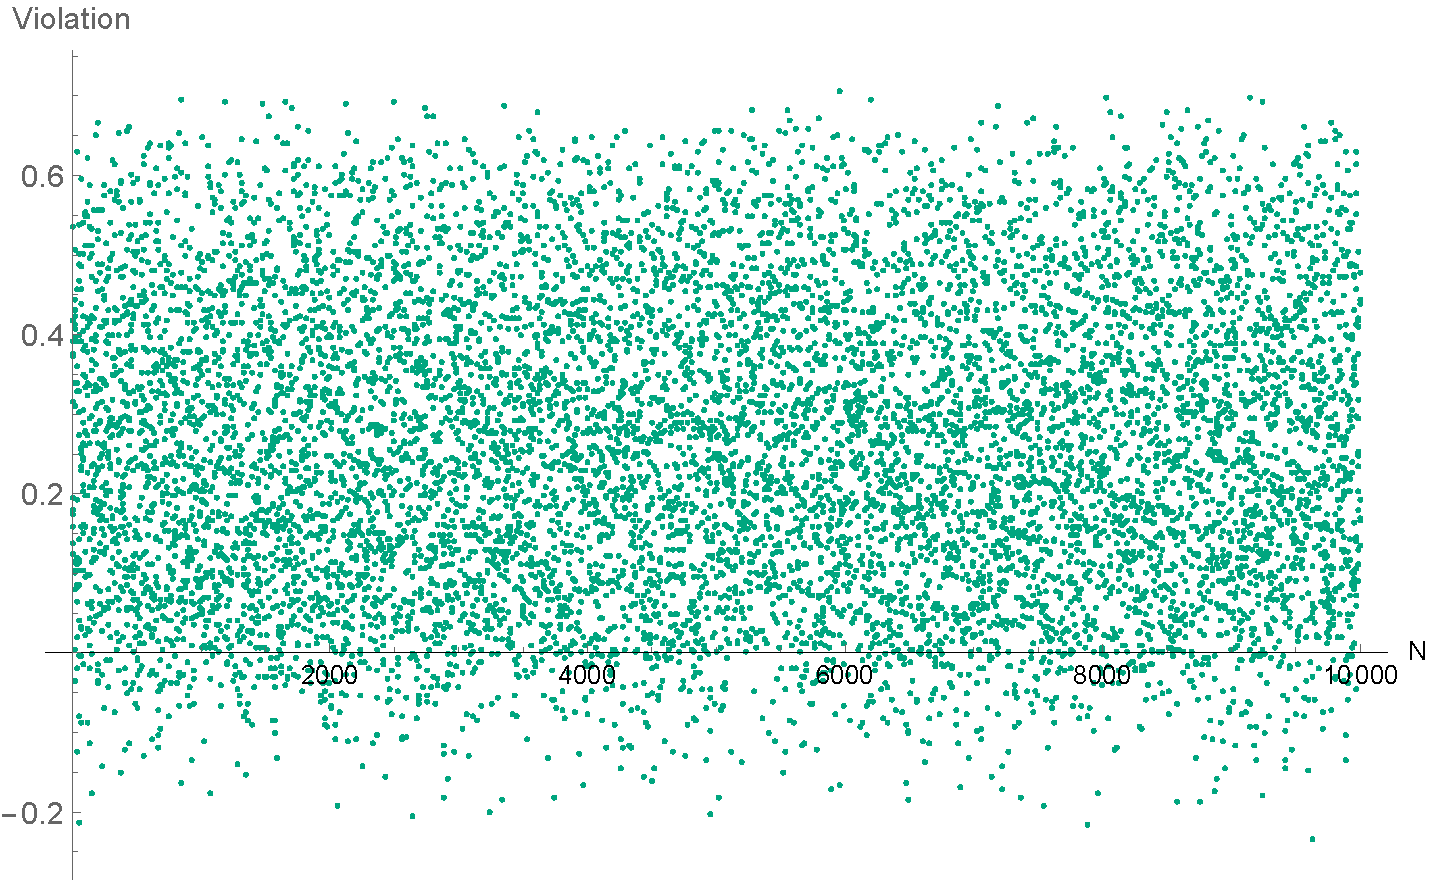
\includegraphics[scale=0.3]{figures/RandomU_p1_3_10k.pdf}}}
\caption{\footnotesize{We plot the LHS of Eq.(\ref{AS_eigenvalue}) for $2\otimes2$ dimension (Violation) against the number of  Haar uniformly generated random unitary matrices (N) for two choices of noise mixing parameter $p$ for modified Werner state.}}
\label{RandomU_modW}
\end{figure}

Now to generalise our result numerically by considering that we have access to one CNOT gate and the other unitary is made completely random. We generate random $100000$ unitary matrices Haar uniformly. Here, we consider two cases corresponding to two initial states, (a) maximally mixed state in $2\otimes2$ dimension i.e. $p=0$ in Eq. (\ref{mod_Wstate}), and (b) $p=1/3$, $\phi=0$, and $\gamma=\pi/4$ in Eq. (\ref{mod_Wstate}), giving us a mixture of white noise with maximally entangled state in $2\otimes2$. For illustration, we plot the cases for $10000$ randomly generated unitary matrices in Fig.(\ref{RandomU_modW}). Note that, both the plots evidently show that it is always possible to find a global unitary operation that makes a AS state a separable one by switching operation with CNOT gate. As can be guessed intuitively, the number of useful unitary matrices to break absolute separability, for Case (b) is more than that for in Case (a) as the state in Case (b) is lying on the boundary of the convex set. We extend our result to higher dimension ($2\otimes d$) by considering maximally mixed state initially while both the random unitary matrices are generated Haar uniformly. We check the absolute separability criterion given in Eq. (\ref{AS_eigenvalue}) and plot the violation. The plots with more details can be found in the appendix.\\
Another interesting observation that can be made from the results of switching action on modified Werner state is about the rank of the final state. The initial state given in Eq. (\ref{mod_Wstate}) is a full-rank state for the whole range of noise mixing parameter $p$. After the switching action, the rank of the final state remains unaltered in most of the cases except for $\theta=\pi/2$ and for odd multiples of $\pi/2$. In these exceptional cases the rank decreases to 2 and making the final state certainly separable as can be seen from Proposition (\ref{prop1}). At the same time, from numerical simulation we find that rank remains unchanged for all the cases. 

\section{Bell diagonal states}

\begin{figure*}[htp]
\centering
\fbox{
\subfigure[Structure of Bell Diagonal states. The octahedron represents the set of separable states \cite{LC_10}, and the inner structure represents the AS states.]{\includegraphics[scale=0.3]{figures/BDstate_AS_Sep_2.pdf}}
%\hfill
\qquad
\subfigure[Structure of BD AS states after switching action for Unitary corresponding to $\theta=\pi/6$]{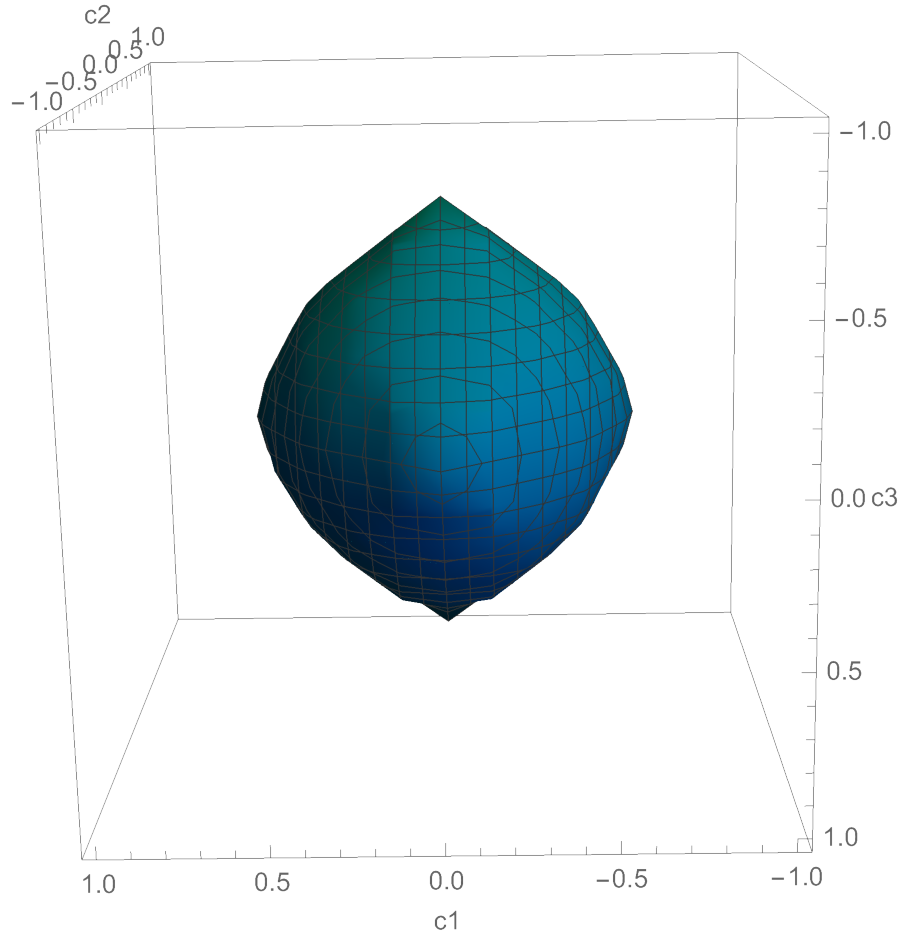
\includegraphics[scale=0.2]{figures/BD_switch_pi_6.pdf}}
\qquad
\subfigure[Structure of BD AS states after switching action for Unitary corresponding to $\theta=\pi/4$]{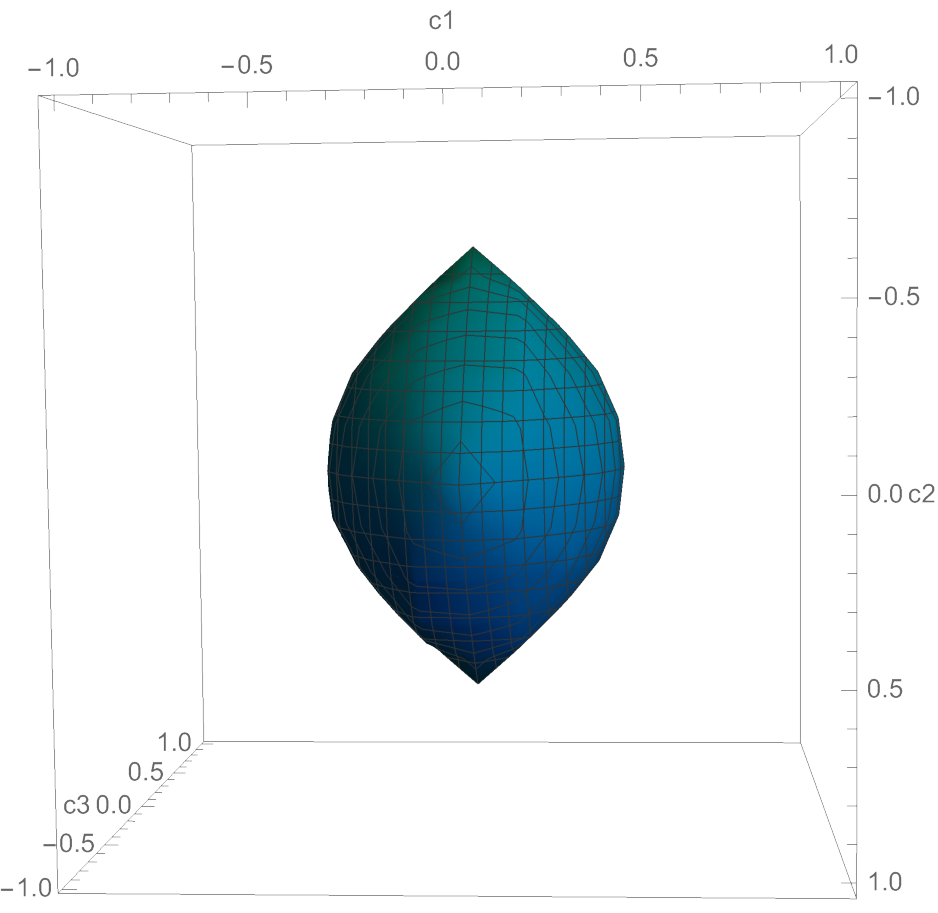
\includegraphics[scale=0.2]{figures/BD_switch_pi_4.pdf}}
\qquad
\subfigure[Structure of BD AS states after switching action for Unitary corresponding to $\theta=\pi/3$]{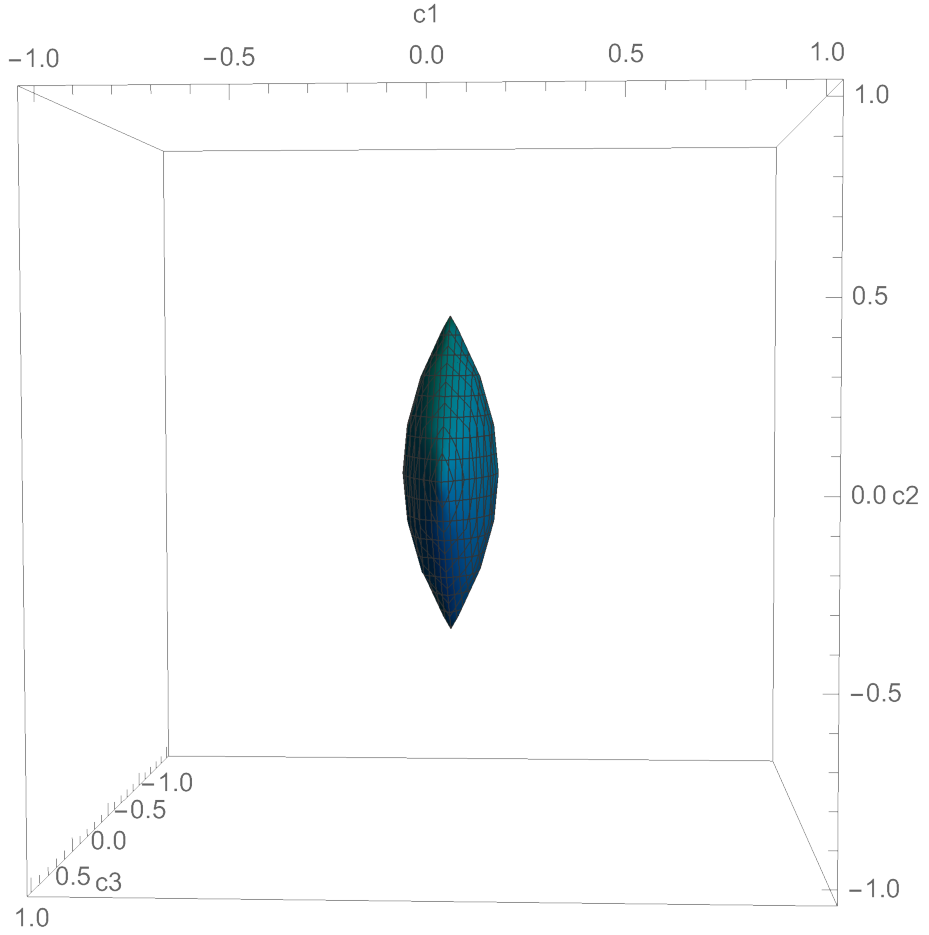
\includegraphics[scale=0.2]{figures/BD_switch_pi_3.pdf}}
}
\caption{\footnotesize{Geometry of BD AS states before and after switching action of global unitary matrices.}}
\label{BD_AS_sep_switch}
\end{figure*}

   % \fbox{\includegraphics[scale=2*0.45]{BDstate_AS_Sep_2.pdf}}
   % \caption{\footnotesize{Structure of Bell Diagonal states. The bigger tetrahedron represents the set of separable states [ref], and the inner structure represents the AS states.}}


Next we move our discussion to the set of Bell-diagonal (BD) states. For that, we first introduce and elaborate the properties of this particular state in the following. The two-qubit Bell diagonal states are the probabilistic mixture of maximally entangled states given in the following form,
\begin{eqnarray}
    \rho_{BD} &=& p_1 \ket{\phi^+}\bra{\phi^+} + p_2 \ket{\phi^-}\bra{\phi^-} + p_3 \ket{\psi^+}\bra{\psi^+} \nonumber \\
    && + p_4 \ket{\psi^-}\bra{\psi^-}
    \label{BD_state_p}
\end{eqnarray}
with, $p_1+p_2+p_3+p_4=1$. Here, $\ket{\phi^{\pm}}=(\ket{00}\pm \ket{11})/\sqrt{2}$ and $\ket{\psi^{\pm}}=(\ket{01}\pm \ket{10})/\sqrt{2}$ are four Bell states. In the Bell-basis, this is a diagonal state. From the partial transposition criterion, it is evident that $\rho_{BD}$ is a separable state if all the mixing probabilities are less than or equal to $1/2$. Note that, the eigenvalues of the state in Eq. (\ref{BD_state_p}) are given by, $\{ p_1, p_2, p_3, p_4\}$. Another form of the state is \cite{LC_10},
\begin{equation}
    \rho_{BD} = \frac{1}{4} (\mathcal{I}+\sum_{i=1}^3 c_i \sigma_i \otimes \sigma_i)
    \label{BD_state_c}
\end{equation}
with $\sigma_i$'s being the Pauli matrices.

\noindent Comparing equations (\ref{BD_state_p}) and (\ref{BD_state_c}), one can get the constraints on the coefficients $c_1$, $c_2$ and $c_3$ which eventually indicates the region describing the separable states and the AS states \cite{LC_10}. For the state to be separable, we have $|c_1|+|c_2|+|c_3| \leq 1$ which gives a tetrahedron structure as illustrated in Fig. (\ref{BD_AS_sep_switch} (a)). Explicitly, $p_1=(1+c_1-c_2+c_3)/4$, $p_2=(1+c_1+c_2-c_3)/4$, $p_3=(1-c_1+c_2+c_3)/4$ and $p_4=(1-c_1-c_2-c_3)/4$. Putting the eigenvalue condition (\ref{AS_eigenvalue}) on these mixing parameters along with the condition of positivity, we find the conditions on $c_1$, $c_2$ and $c_3$ for $\rho_{BD}$ to be an AS state which enables us to obtain the structure of AS states as also illustrated in Fig. (\ref{BD_AS_sep_switch} (a)). 
\begin{result}
    If the initial state is $\rho_{BD}$ given in Eq.(\ref{BD_state_c}) and it undergoes the switching operation between two unitary channels, one being CNOT and the other given in Eq. (\ref{unitary_theta}), then it is possible to change the structure of the set of AS BD states for varying the parameter $\theta$ in Eq. (\ref{unitary_theta}) as shown in Fig. (\ref{BD_AS_sep_switch} (b), (c), (d)). 
\end{result}
For the understanding of the result we refer to Fig. (\ref{BD_AS_sep_switch}). Let us now note some observations that can be made from the mentioned figure. Firstly, the size of the set of AS BD states decreases with the increasing $\theta$ value. Eventually, it can been seen for $\theta=\pi/2$ the set completely vanishes which implies that all the BD AS states can be made atleast separable under suitable choice of global unitary matrices.

\begin{figure*}[htp]
\centering
\fbox{
\subfigure[BD states for $\alpha=0.17$ to $0.5$. Here, $N=(\alpha-0.17)/0.01$.]{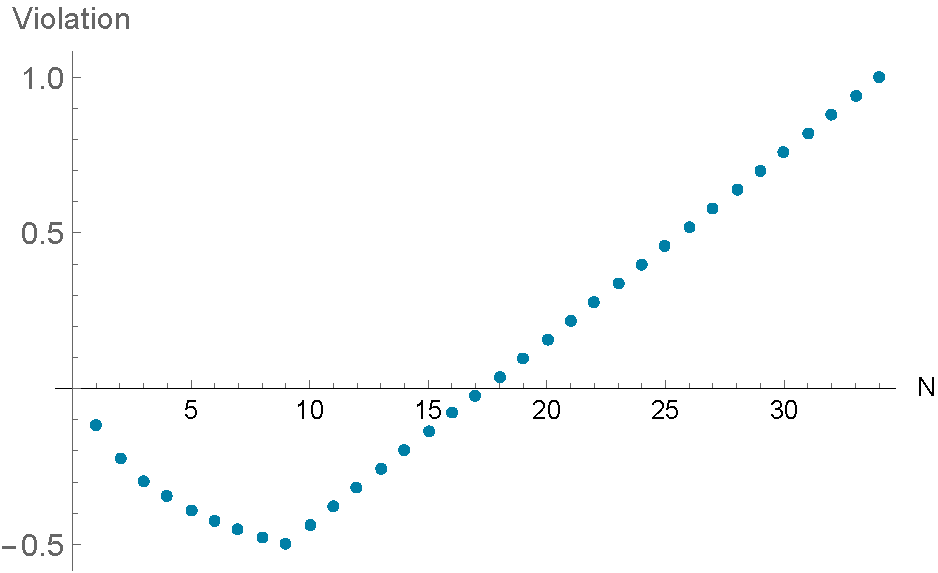
\includegraphics[scale=0.22]{figures/BD_3_alpha_vio.pdf}}
%\hfill
\qquad
\subfigure[For $\alpha=0.18$ after Switching action. (Here, $N$ is number of random unitary.)]{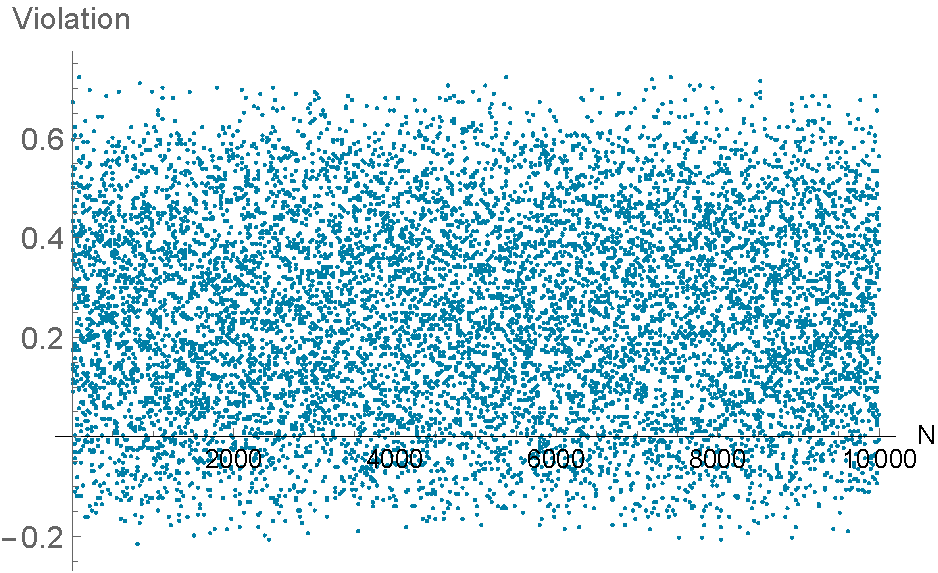
\includegraphics[scale=0.22]{figures/BD_3_alpha_0.18_switch.pdf}}
\qquad
\subfigure[For $\alpha=0.20$ after Switching action. (Here, $N$ is number of random unitary.)]{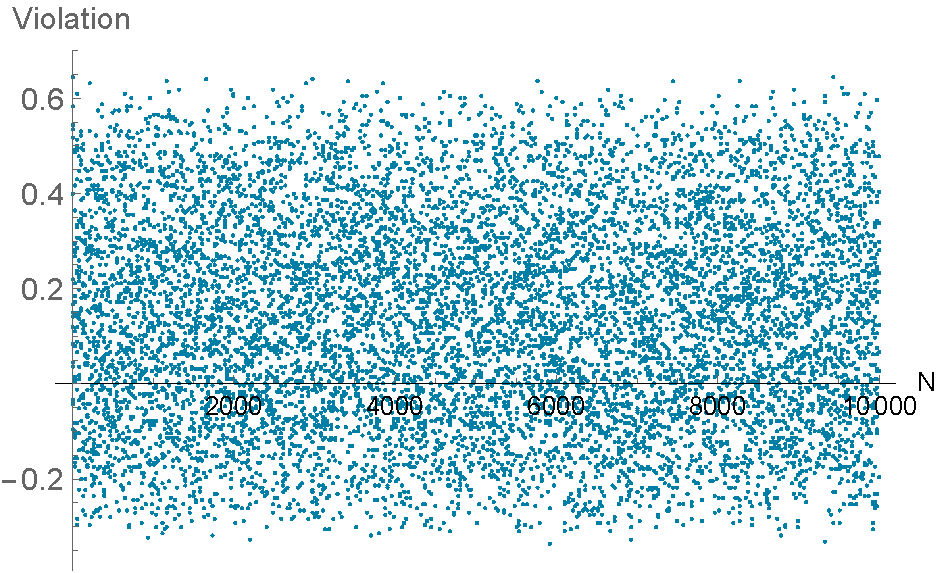
\includegraphics[scale=0.22]{figures/BD_3_alpha_0.2_switch.pdf}}
\qquad
\subfigure[For $\alpha=0.26$ after Switching action. (Here, $N$ is number of random unitary.)]{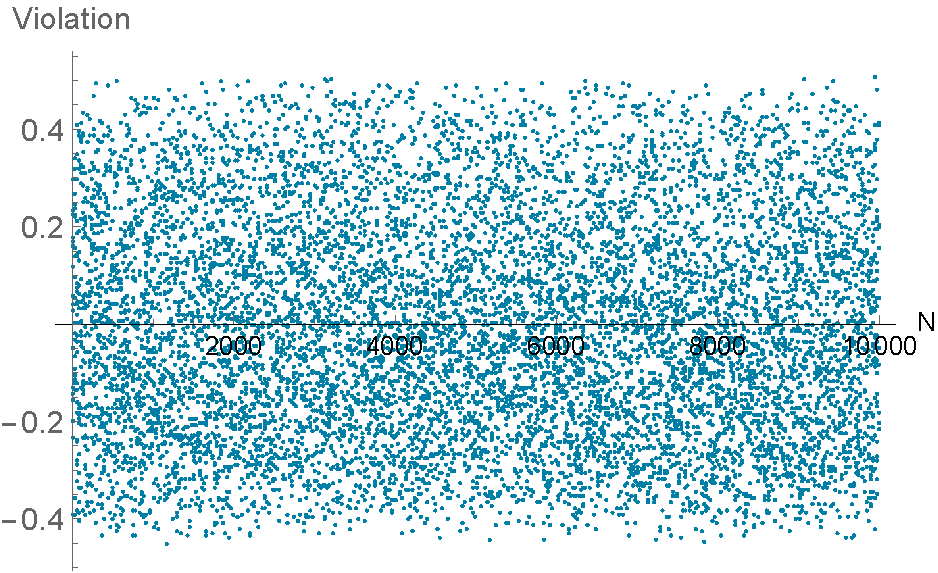
\includegraphics[scale=0.22]{figures/BD_3_alpha_0.26_switch.pdf}}}
\caption{\footnotesize{A particular type of BD state and Switching action of random unitary and CNOT gate on them.}}
\label{BD_random}
\end{figure*}

Now let us consider a particular case of BD state. We choose, three of the mixing parameter having the same value i.e. $p_2=p_3=p_4=\frac{1}{2}-\alpha$ making, $p_1=3\alpha-1/2$ with $\alpha$ running from $1/6$ to $1/2$. In this case, we plot the eigenvalue condition given in Eq. (\ref{AS_eigenvalue}) to find the range for AS states as shown in Fig. (\ref{BD_random}(a)). Then for some particularly chosen values of $\alpha$ we take CNOT gate along with a randomly generated unitary (Haar uniformly generated) and check the switching action on the given state as shown in Fig. (\ref{BD_random} (b), (c), (d)). It is clear from the plots that as $\alpha$ increases, the number of effective unitary matrices (though there always exists many) decreases. It is intuitive as from plot (a) in Fig. (\ref{BD_random}) the lower values of $\alpha$ are nearer to the boundary of the set of AS states. 


%\textcolor{blue}{If possible please workout this as a toy example with the help of fixed $U$ and $\alpha$ by calculating the condition.}



\section*{Results on higher dimensions}
\noindent  For the dimensions $2\otimes d$ we consider the maximally mixed state i.e. $\mathcal{I}_{2\otimes d}/2d$ as the initial state. This is definitely AS and moreover this is a free state in every resource theory. Then we Haar uniformly generate two unitary matrices and use them in switching action on the initial state. We explicitely deal with three cases of dimensions $2\otimes 3$, $2 \otimes 4$, and $2 \otimes 10$. The cases are plotted in Fig. (\ref{higher_d}). From the figure, it is evident that even in higher dimension where the condition given in Eq. (\ref{AS_eigenvalue}) holds, it is possible to find numerous number of global unitary matrices which can make AS states resourceful. Note that, the criterion stated in Eq. (\ref{finalstate_switch}) remains unchanged in these cases. 

\begin{figure*}[htp]
\centering
\fbox{
\subfigure[For $2\otimes 3$ dimension.]{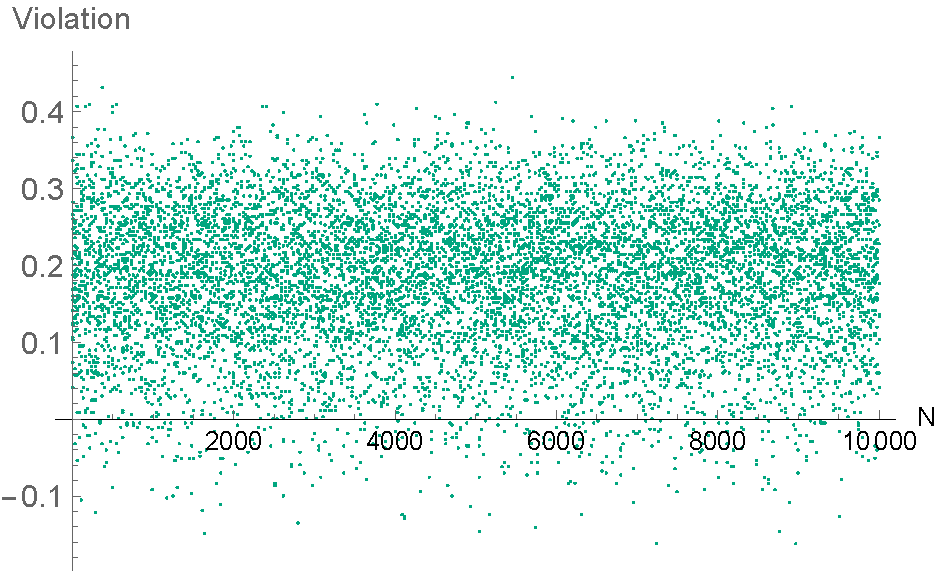
\includegraphics[scale=0.32]{figures/RandomU_2_3.pdf}}
%\hfill
\qquad
\subfigure[For $2\otimes 4$ dimension.]{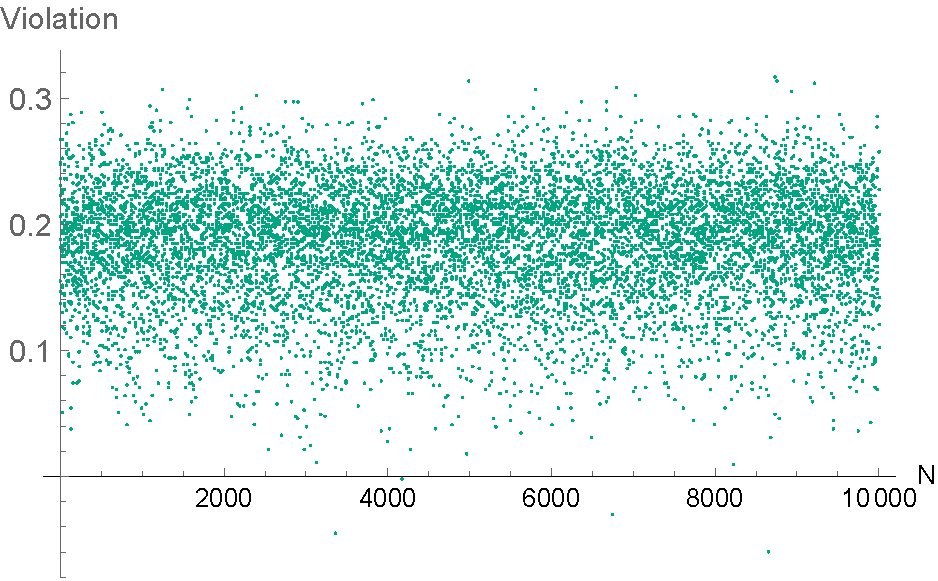
\includegraphics[scale=0.32]{figures/RandomU_2_4.pdf}}
\qquad
\subfigure[For $2\otimes 10$ dimension.]{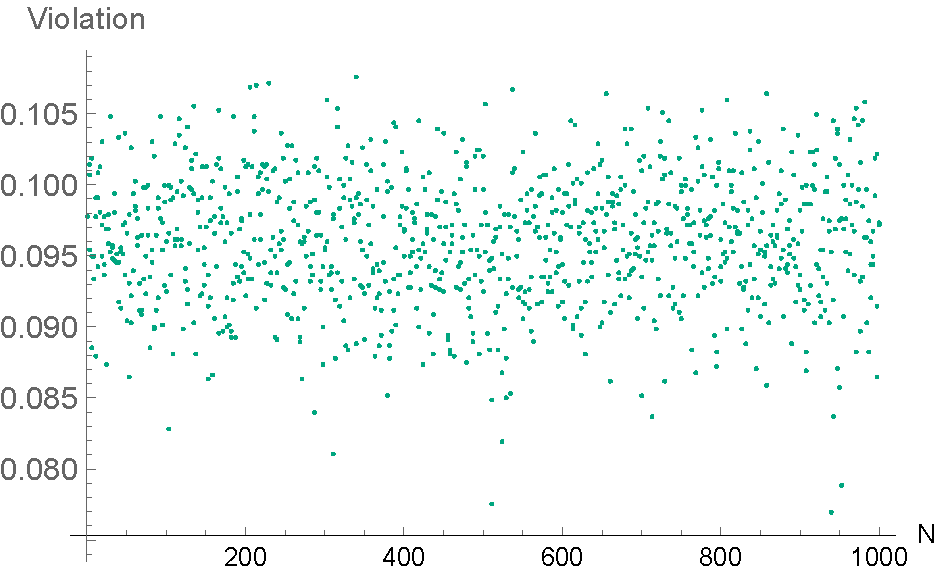
\includegraphics[scale=0.32]{figures/RandomU_2_10.pdf}}}
\caption{\footnotesize{Breaking absolute separability in higher dimensions. The axes have their usual meaning.}}
\label{higher_d}
\end{figure*}


